\documentclass[conference]{IEEEtran}
\usepackage[T1]{fontenc}
\usepackage{listings}
\usepackage{graphicx}
\usepackage{url}
\usepackage{array}
\usepackage{booktabs}
\setlength{\tabcolsep}{4pt}
\newcolumntype{P}[1]{>{\raggedright\arraybackslash}p{#1}}
\lstset{basicstyle=\ttfamily\footnotesize,breaklines=true,columns=fullflexible,frame=single,keepspaces=true,showstringspaces=false}
\newcommand{\code}[1]{\texttt{#1}}
\title{Logic Lab: A Logic Gates Compiler with Interactive Phase Visualization}
\author{\IEEEauthorblockN{Dibyajyoti, Rhythm Jain, Prince Sahoo, Ritik Raj, A M YEESHU}
\IEEEauthorblockA{Team ABC --- Compiler Design Project\\
CS \& AI, Rishihood University}}
\begin{document}
\maketitle
\begin{abstract}
Logic Lab is a compiler design project that turns Boolean source code into a logic circuit, Verilog code, and a truth table. It shows the output of each compiler phase so that students can understand how the source becomes a working circuit. The backend is written in Python, and the frontend uses React and TypeScript. The compiler checks tokens, grammar, declarations, assignments, and circuit dependencies. It then creates intermediate code, applies simple optimizations, and generates the target code. The interface shows tokens, an abstract syntax tree, a symbol table, intermediate instructions, optimization steps, and the generated circuit. Users can change input bits and see the output change. The automated tests passed 62 cases; two checks that require an external Verilog simulator were skipped. This report explains the design, a complete worked example, error handling, test results, assigned team responsibilities, AI assistance, and future improvements.
\end{abstract}
\begin{IEEEkeywords}
compiler design, logic gates, Boolean expressions, Verilog, interactive visualization
\end{IEEEkeywords}

\section{Introduction}
A compiler translates a program from one language into another form. It normally works through several phases, including lexical analysis, syntax analysis, semantic analysis, intermediate code generation, optimization, and code generation~\cite{aho}. Students often study these phases separately. This project brings them together in one application and makes their inputs and outputs visible.

Logic gates are a useful compiler use case because their operations are small enough to understand, but they still need real language rules. A source expression must have valid tokens and grammar. Every signal must be declared, and the circuit must not contain an invalid dependency cycle. The final circuit must also produce the correct output for each input combination.

Logic Lab is more than a Boolean calculator. It translates source code into a different target language, Verilog, and a gate netlist. A netlist is a list of gates and their connections. The truth table and live circuit view help users check this translation.

\section{Problem Statement and Objectives}
The project solves the following problem: accept a small logic-gate program, check that it is valid, translate it into a circuit, and explain every step of that translation.

The main objectives are:
\begin{enumerate}
\item Implement all six core compiler phases in Python.
\item Show tokens, the abstract syntax tree (AST), the symbol table, intermediate representation (IR), optimization changes, and target code.
\item Generate a correct circuit and truth table for valid programs.
\item Report lexical, syntax, and semantic errors with source locations.
\item Keep modules separate so that each team member can explain a clear input/output contract.
\item Provide setup instructions, tests, a report, and viva preparation material in one repository.
\end{enumerate}

The selected scope is \emph{combinational logic}. Outputs depend on the current inputs only. Clocks, stored state, flip-flops, and timing delays are outside the current scope. Supported examples include a half adder, a full adder, a multiplexer, and circuits with shared intermediate expressions.

\section{Methodology and System Design}
\subsection{Technology Stack}
Python implements the compiler. FastAPI exposes it through an HTTP API. React and TypeScript implement the interface, while CodeMirror provides the source editor~\cite{codemirror}. Vite builds the frontend into static files. Pytest checks the Python implementation. Git and GitHub store the source and change history.

The frontend and backend are in the same repository, but they run separately. The frontend can be hosted as a static website; compilation still requires the Python API. No AI model is called while a user compiles a program.

\subsection{Architecture}
Figure~\ref{fig:pipeline} shows the main data flow. Each phase is a separate Python module. The compiler modules do not depend on React or FastAPI, so they can also be used from the command line.
\begin{figure}[ht]
\centering
\fbox{\begin{minipage}{0.89\columnwidth}
\centering
Source code\\$\downarrow$\\
Lexer $\rightarrow$ Tokens\\$\downarrow$\\
Parser $\rightarrow$ AST\\$\downarrow$\\
Semantic analysis $\rightarrow$ Symbols and order\\$\downarrow$\\
IR generation $\rightarrow$ Three-address code\\$\downarrow$\\
Optimization $\rightarrow$ Improved IR\\$\downarrow$\\
Code generation $\rightarrow$ Verilog and netlist\\$\downarrow$\\
Simulation $\rightarrow$ Truth table and live values
\end{minipage}}
\caption{Compiler workflow. Simulation checks and displays the generated result; it is an additional stage after code generation.}
\label{fig:pipeline}
\end{figure}

\subsection{API and Phase Contracts}
The frontend sends source code and an optimization option to \code{POST /api/compile}. The response includes a schema version, a success flag, phase results, and diagnostics. A phase result contains its input, output, status, and explanation. \code{GET /api/health} checks whether the server is running.

A language error does not remove earlier successful results. For example, a semantic error leaves the tokens and AST available, while IR and later stages are marked blocked. Invalid API request shapes are rejected separately from errors in the source language.

\begin{table}[ht]
\caption{Module Inputs and Outputs}
\label{tab:contracts}
\centering\small
\begin{tabular}{@{}P{0.22\columnwidth}P{0.28\columnwidth}P{0.43\columnwidth}@{}}
\toprule
Module & Input & Output\\\midrule
Lexer & Source string & Tokens and locations\\
Parser & Token list & AST and parse trace\\
Semantic & AST & Symbols, dependencies, ordered assignments\\
IR generation & Validated program & Three-address instructions\\
Optimizer & Original IR & Optimized IR and rewrite log\\
Code generator & Selected IR & Verilog, netlist, port map\\
Simulator & Netlist & Truth-table columns and rows\\\bottomrule
\end{tabular}
\end{table}

\section{Source Language}
\subsection{Basic Syntax}
The language supports \code{INPUT}, \code{WIRE}, and \code{OUTPUT} declarations. Every signal holds one bit. Statements end with semicolons, and declarations must appear before assignments. Identifiers are case-sensitive, while keywords are uppercase. A comment starts with \code{//} and ends at the end of its line.

The supported gates are AND, OR, NOT, NAND, NOR, XOR, and XNOR. The constants are 0 and 1. The following valid program is used throughout this report:
\begin{lstlisting}
INPUT a, b, c;
WIRE intermediate;
OUTPUT out;
intermediate = a AND b;
out = intermediate OR NOT c;
\end{lstlisting}

\subsection{Grammar and Precedence}
The main grammar is shown below. Braces mean repetition, and the vertical bar means a choice.
\begin{lstlisting}
program = {declaration} {assignment}
declaration = (INPUT | WIRE | OUTPUT)
              identifier {, identifier} ;
assignment = identifier = expression ;
expression = xor_expr {(OR | NOR) xor_expr}
xor_expr = and_expr {(XOR | XNOR) and_expr}
and_expr = unary {(AND | NAND) unary}
unary = NOT unary | (expression)
        | identifier | 0 | 1
\end{lstlisting}
NOT has the highest precedence, then AND/NAND, XOR/XNOR, and OR/NOR. Parentheses can change the grouping. Binary operators at the same level are grouped from left to right. This matters for NAND and NOR because changing their grouping can change the result.

\subsection{Semantic Rules and Limits}
Every referenced signal must be declared. Names cannot be declared twice. Inputs cannot be assigned. Every wire and output must be assigned exactly once, and a program must declare at least one output. A reference to a later assignment is allowed if the complete dependency graph has no cycle.

The compiler accepts at most 20,480 UTF-8 source bytes, 12 input signals, and 200 declared signals. Expression nesting and AST height are limited to 64. Twelve inputs produce 4096 truth-table rows. These limits keep the demo manageable and prevent very large truth tables from overwhelming the interface.

\section{Compiler Implementation}
\subsection{Lexical Analysis}
The lexer reads the source from left to right and groups characters into tokens. It recognizes complete identifiers before checking whether they are keywords. For example, \code{AND} is a keyword, while \code{ANDY} is an identifier. Whitespace and comments are skipped, but the source position is still updated.

Each token stores its type, original text, and location. For example, \code{out = a AND b;} produces IDENT, EQUAL, IDENT, AND, IDENT, and SEMI tokens. An explicit EOF token marks the end. A character such as \code{\&} is rejected because the language uses the word AND rather than that symbol.

\subsection{Syntax Analysis}
The parser uses recursive descent and precedence climbing. Recursive descent means that small functions recognize parts of the grammar. Precedence climbing decides which operator should group first. The result is an AST: a tree that keeps the meaningful operators and operands without unnecessary punctuation.

For the worked example, the output expression has OR at its root. Its left child is the reference \code{intermediate}, and its right child is NOT with child \code{c}. The parser also records a short trace of completed declarations and assignments. Missing parentheses, missing semicolons, and missing operands are syntax errors.

\subsection{Semantic Analysis}
Semantic analysis checks meaning after the grammar is accepted. It builds a symbol table, checks declaration and assignment rules, and collects the signals used by each expression.

The dependencies form a graph. A depth-first search puts each assignment after the signals it needs. This is called a topological order. During the search, revisiting a signal that is still being explored identifies a cycle. A program such as \code{w = out; out = w;} is therefore rejected, even if both names are declared.

\subsection{Intermediate Code Generation}
The IR generator visits child expressions before their parent operation. It creates a temporary for each gate and then a COPY instruction for the named assignment. An instruction stores a destination, an operation, operands, and a source location.

This simple form is often called three-address code: an operation uses up to two input values and stores one result. Temporary names begin with \code{\%}, which cannot appear in a user identifier. Keeping IR separate allows optimization and code generation to work without reparsing the source.

\subsection{Optimization}
The optimizer applies small changes that preserve the outputs:
\begin{itemize}
\item Constant folding: calculate expressions such as \code{1 AND 0} during compilation.
\item Boolean identities: replace \code{a AND 1} with \code{a}, or \code{a OR 0} with \code{a}.
\item Double negation: replace \code{NOT NOT a} with \code{a}.
\item Copy propagation: use the original value instead of an unnecessary intermediate copy.
\item Common-subexpression elimination: reuse a result when the same gate operation is computed again.
\item Dead-code elimination: remove internal computations that cannot affect any output.
\end{itemize}
The application records the rule and the before/after values for every rewrite. Public input and output names are preserved. These are local optimizations; the project does not claim to find the smallest possible circuit.

\subsection{Code Generation}
The code generator converts the selected IR into Verilog and a structural netlist. Verilog is a language for describing digital hardware. Boolean operations become gate primitives, and COPY becomes a continuous assignment.

Source names are mapped to safe names such as \code{s0} and \code{s1}. This avoids conflicts with Verilog keywords. A port map explains the correspondence between the original names and the generated names. The netlist retains the logical names and is used to draw the circuit.

\subsection{Simulation}
The simulator tries every combination of input bits. It evaluates gates in dependency order and collects the output values into a truth table. A circuit with no inputs and one constant output has one row. The frontend also evaluates the netlist when the user toggles an input.

For $n$ inputs and $I$ instructions, a full truth table requires about $2^n I$ gate-evaluation steps. This explains why truth-table generation becomes expensive as the number of inputs grows.

\section{Worked Example and Output}
\subsection{Tokens, AST, and Symbols}
For the statement \code{intermediate = a AND b;}, the lexer produces six tokens before the final EOF of the program. The parser represents this assignment as an AND node with reference children a and b. Table~\ref{tab:symbols} shows the symbol table for the complete example.
\begin{table}[ht]
\caption{Symbol Table for the Worked Example}
\label{tab:symbols}
\centering\small
\begin{tabular}{lll}
\toprule Signal & Kind & Depends on\\\midrule
a & INPUT & --\\b & INPUT & --\\c & INPUT & --\\
intermediate & WIRE & a, b\\out & OUTPUT & intermediate, c\\\bottomrule
\end{tabular}
\end{table}
The semantic order is intermediate followed by out. The AST does not itself prove that these references are valid; that is the job of the symbol and dependency checks.

\subsection{Original and Optimized IR}
The original IR contains five instructions:
\begin{lstlisting}
%0 = AND a, b
intermediate = COPY %0
%2 = NOT c
%3 = OR intermediate, %2
out = COPY %3
\end{lstlisting}
After copy propagation, it contains four:
\begin{lstlisting}
%0 = AND a, b
%2 = NOT c
%3 = OR %0, %2
out = COPY %3
\end{lstlisting}
Temporary numbers can have gaps because the generator counts all instructions, including copies. Removing one COPY reduces the IR count, but it does not mean that a physical Boolean gate was removed: COPY becomes wiring in Verilog.

\subsection{Generated Verilog}
The input ports a, b, c map to s0, s1, s2, and out maps to s3. The generated target is:
\begin{lstlisting}
module logic_circuit(s0, s1, s2, s3);
  input s0, s1, s2;
  output s3;
  wire s4, s5, s6;
  and g0 (s4, s0, s1);
  not g1 (s5, s2);
  or g2 (s6, s4, s5);
  assign s3 = s6;
endmodule
\end{lstlisting}
Figure~\ref{fig:circuit} shows the same three-gate circuit. The figure is a schematic of the worked example, not a browser screenshot.
\begin{figure}[ht]
\centering
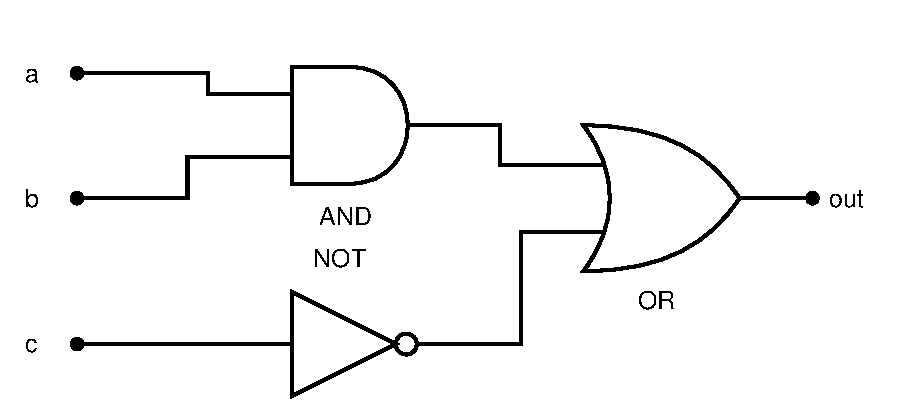
\includegraphics[width=\columnwidth]{circuit-example.pdf}
\caption{Circuit for $out=(a\land b)\lor\neg c$. AND combines a and b; NOT inverts c; OR produces out.}
\label{fig:circuit}
\end{figure}

\subsection{Truth Table}
Table~\ref{tab:truth} lists every input combination. When c is 0, NOT c is 1, so out is 1. When c is 1, out equals a AND b.
\begin{table}[ht]
\caption{Truth Table for the Worked Example}
\label{tab:truth}
\centering
\begin{tabular}{cccc}
\toprule a & b & c & out\\\midrule
0&0&0&1\\0&0&1&0\\0&1&0&1\\0&1&1&0\\
1&0&0&1\\1&0&1&0\\1&1&0&1\\1&1&1&1\\\bottomrule
\end{tabular}
\end{table}

\section{Interactive Visualization}
The source editor is on the left, and phase results are on the right. Each phase has Input, Output, Explanation, and JSON views. The Input view shows exactly what the module receives, while Output shows its result. The AST can be expanded, and tables present tokens and symbols clearly.

After a successful compilation, the Circuit tab opens automatically. It draws conventional gate symbols and connected wires from the generated netlist. Green wires carry 1 and gray wires carry 0. Users can toggle input bits, inspect named outputs, switch between fit and actual size, and export an SVG. Verilog and netlist JSON can also be downloaded. The simulation view offers a paginated truth table and CSV export.

If source code changes, previous results are marked outdated until the next compilation. A newer request cannot be overwritten by an older response. The offending text is underlined in the editor until the source changes, and clicking a diagnostic selects its source location. On narrow screens, the editor and results are stacked vertically.

\section{Error Handling and Quality Checks}
\subsection{Errors by Phase}
Table~\ref{tab:errors} gives examples of invalid input. The current compiler reports the first language error, then stops the later phases. Users correct the source and compile again.
\begin{table}[ht]
\caption{Important Error Cases}
\label{tab:errors}
\centering\small
\begin{tabular}{@{}P{0.19\columnwidth}P{0.39\columnwidth}P{0.35\columnwidth}@{}}
\toprule Phase & Example problem & Expected handling\\\midrule
Lexical & Unsupported character \code{\&} & Invalid-character diagnostic\\
Syntax & Missing semicolon or operand & Expected-token or expression diagnostic\\
Syntax & Unclosed parenthesis & Expected closing token\\
Semantic & Undeclared signal & Undefined-signal diagnostic\\
Semantic & Duplicate declaration & Reject reused name\\
Semantic & Output assigned twice & Reject second assignment\\
Semantic & Assignment to an input & Reject assignment\\
Semantic & Wire/output never assigned & Missing-assignment diagnostic\\
Semantic & Dependency cycle & Cycle diagnostic\\
Limits & Too many inputs or deep expression & Clear limit diagnostic\\\bottomrule
\end{tabular}
\end{table}

\subsection{Testing Method}
Unit tests check each phase and its edge cases. Integration tests run full programs through the pipeline and check the API contract. Test programs include all seven gates, constants, multiple outputs, forward references, adders, and a multiplexer.

The optimizer is also tested with 150 generated programs. Each has three inputs and two outputs, and all eight input combinations are checked. A separate AST evaluator gives the expected result. The tests compare this result with the original IR, optimized IR, and generated netlist. This produces 1200 input-vector checks across the generated programs. It gives evidence for these cases; it is not a proof for every possible program.

\subsection{Recorded Results}
\begin{table}[ht]
\caption{Verified Results and Limits}
\label{tab:results}
\centering\small
\begin{tabular}{@{}P{0.57\columnwidth}P{0.36\columnwidth}@{}}
\toprule Check & Recorded result\\\midrule
Python automated tests & 73 passed, 0 skipped\\
External Verilog simulator tests & Passed\\
Random programs vs. independent evaluator & 3000 checked\\
Generated Verilog co-simulation & 240 runs matched\\
Generated program input vectors & 1200 checked\\
Maximum truth-table rows & 4096 checked\\
TypeScript and static frontend build & Passed\\
Fresh local clone: tests and build & Passed\\
Optimization demo: IR count & 9 reduced to 2\\
Introduction example: IR count & 5 reduced to 4\\\bottomrule
\end{tabular}
\end{table}
The external Verilog tests use Icarus Verilog~\cite{icarus} (version 13.0). They simulate the generated Verilog and compare every output with the compiler's own truth table; they pass. A separate review compiled 240 Verilog modules, from 120 random programs with optimization on and off, with a testbench that tries every input combination. All outputs matched an independent evaluator. This is strong evidence for the tested programs, not a proof for every possible program.

Browser checks confirmed compilation, AST display, diagnostic selection, live circuit values, the optimization log, and the full-adder truth table. All gate outputs were also checked in the circuit view for input vectors 00, 11, and 10. A Verilog download succeeded. Fit/actual-size switching worked, and a 390-pixel viewport had no document-level horizontal overflow. No browser recording was required for the circuit update.

\section{Individual Member Contributions}
Table~\ref{tab:members} lists the agreed module ownership. Full member names are shown below; the account mapping is recorded in the repository contribution guide. The repository contains separate module commits using these authorized identities.
\begin{table}[ht]
\caption{Assigned Team Responsibilities}
\label{tab:members}
\centering\small
\begin{tabular}{@{}P{0.28\columnwidth}P{0.65\columnwidth}@{}}
\toprule Member identity & Assigned module and deliverables\\\midrule
Dibyajyoti (Dibya-z) & Lexer, positioned tokens, token view, language specification, lexer tests\\
Rhythm Jain & Parser, precedence rules, AST, AST view, parser tests\\
Prince Sahoo & Semantic checks, symbol table, dependency order, diagnostics, semantic tests\\
Ritik Raj & IR generation, optimization rules, rewrite view, equivalence tests\\
A M YEESHU & Code generation, Verilog, simulation, circuit view, frontend/backend integration\\\bottomrule
\end{tabular}
\end{table}

\subsection{Actual Work and Review Status}
The team representative chose the topic, stack, requirements, ownership split, and local-first workflow. An AI coding assistant produced the initial source code, tests, interface, documentation, and report draft, and ran the recorded checks. Individual student implementation, testing, and review have not yet been confirmed in the project record.

The table is therefore an ownership breakdown, not a claim that each student independently wrote every assigned file. Each member must review the module, run its tests, explain its input and output, and record actual changes or review evidence before submission. Pending reviews are tracked in \code{docs/contributions.md}. Git author metadata alone is not proof of independent implementation.

\section{AI Assistance and Reproducibility}
The project uses the rubric's AI Product Engineering track. AI assisted development and documentation, but the final compiler is deterministic Python. It does not send source to a language model at runtime, and it does not execute source through Python eval or exec.

The repository includes the frontend, backend, examples, dependency lockfiles, tests, phase guides, and README setup commands. The main verification commands are:
\begin{lstlisting}
.venv/bin/python -m pytest -q
npm --prefix frontend run build
\end{lstlisting}
The project repository is listed in the references~\cite{repo}. It is publicly accessible at the time of this report. The report uses the IEEE conference document class and two-column layout~\cite{ieee}.

\section{Limitations and Future Scope}
Current limits include single-bit signals, combinational logic only, one reported error at a time, and a maximum of 12 inputs for complete truth tables. Optimization uses a selected set of local rules. Large circuit drawings may need scrolling, and the generated Verilog has been simulated only for the tested programs and a simple testbench; it has not been synthesized for hardware.

Possible improvements are:
\begin{enumerate}
\item Add more Boolean simplification rules and formal equivalence checks.
\item Generate other targets, such as VHDL or additional netlist formats.
\item Improve parser recovery so that one compile can report several errors.
\item Support buses and larger circuits without listing every truth-table row.
\item Improve circuit layout to reduce wire crossings.
\item Add sequential logic only after defining clear clock and state rules.
\end{enumerate}
Optimization is already implemented; future work would extend it rather than add it for the first time.

\section{Conclusion}
Logic Lab implements the full compiler pipeline for a small Boolean language. It checks source code, creates and optimizes IR, and generates Verilog and a circuit netlist. The interface makes every phase visible and lets users test the circuit through input switches and truth tables. The project supports both compiler learning and an end-to-end viva demonstration. Its test results, current limits, AI assistance, and pending member reviews are stated openly so that the report matches the implementation.

\begin{thebibliography}{9}
\bibitem{aho} A. V. Aho, M. S. Lam, R. Sethi, and J. D. Ullman, \emph{Compilers: Principles, Techniques, and Tools}, 2nd ed. Pearson, 2006.
\bibitem{codemirror} CodeMirror, ``System guide.'' [Online]. Available: \url{https://codemirror.net/docs/guide/}
\bibitem{icarus} Icarus Verilog, ``Icarus Verilog documentation.'' [Online]. Available: \url{https://steveicarus.github.io/iverilog/}
\bibitem{repo} Logic Lab team, ``Logic-Gates-Compiler source repository.'' [Online]. Available: \url{https://github.com/codic-yeeshu/Logic-Gates-Compiler}
\bibitem{ieee} IEEE, ``Conference manuscript templates.'' [Online]. Available: \url{https://www.ieee.org/conferences/publishing/templates.html}
\end{thebibliography}
\end{document}
